%=========================================================================
%  Presentación de defensa — TFM David Quinzaños Saiz
%  Búsqueda de factores RSA compartidos: Binary Tree Batch GCD
%  Tema UC a medida (sin paquetes de tema externos). Compilar con pdflatex.
%=========================================================================
\documentclass[aspectratio=169,11pt]{beamer}

\usepackage[T1]{fontenc}
\usepackage[utf8]{inputenc}
\usepackage[spanish,es-noshorthands]{babel}
\usepackage{lmodern}
\usepackage{amsmath,amssymb}
\usepackage{graphicx}
\usepackage{booktabs}
\usepackage{tikz}
\usetikzlibrary{arrows.meta,positioning,shapes.geometric,calc}

\graphicspath{{../figuras/}{../resultados/benchmark/}{../resultados/ctlogs/}}

%--------------------------- Paleta UC -----------------------------------
\definecolor{ucazul}{RGB}{0,48,99}
\definecolor{ucgranate}{RGB}{124,20,40}
\definecolor{ucgris}{RGB}{95,95,95}
\definecolor{ucclaro}{RGB}{233,238,244}
\definecolor{ucverde}{RGB}{0,120,90}

%--------------------------- Tema a medida -------------------------------
\setbeamercolor{normal text}{fg=black!88}
\setbeamercolor{structure}{fg=ucazul}
\setbeamercolor{frametitle}{fg=white,bg=ucazul}
\setbeamercolor{title}{fg=ucazul}
\setbeamercolor{alerted text}{fg=ucgranate}
\setbeamercolor{block title}{fg=white,bg=ucazul}
\setbeamercolor{block body}{fg=black!88,bg=ucclaro}
\setbeamercolor{itemize item}{fg=ucgranate}
\setbeamercolor{itemize subitem}{fg=ucazul}
\setbeamercolor{section in toc}{fg=ucazul}

\setbeamerfont{frametitle}{series=\bfseries,size=\large}
\setbeamerfont{title}{series=\bfseries,size=\LARGE}
\setbeamerfont{block title}{series=\bfseries}

\setbeamertemplate{navigation symbols}{}
\setbeamertemplate{itemize item}{\small\raisebox{0.15ex}{\textcolor{ucgranate}{\rule{1.1ex}{1.1ex}}}}
\setbeamertemplate{itemize subitem}{\textcolor{ucazul}{\textbf{--}}}
\setbeamertemplate{blocks}[rounded][shadow=false]

% Barra de título con franja granate inferior
\setbeamertemplate{frametitle}{%
  \nointerlineskip
  \begin{beamercolorbox}[wd=\paperwidth,ht=2.6ex,dp=1.1ex,leftskip=0.5cm,rightskip=0.5cm]{frametitle}%
    \usebeamerfont{frametitle}\insertframetitle%
  \end{beamercolorbox}%
  \nointerlineskip
  \begin{beamercolorbox}[wd=\paperwidth,ht=0.5ex,dp=0ex]{}%
    \hspace*{0pt}\textcolor{ucgranate}{\rule{\paperwidth}{0.5ex}}%
  \end{beamercolorbox}%
}

% Pie de página
\setbeamertemplate{footline}{%
  \leavevmode%
  \hbox{%
  \begin{beamercolorbox}[wd=.40\paperwidth,ht=2.4ex,dp=1ex,leftskip=.3cm]{}%
    \tiny\textcolor{ucgris}{D. Quinzaños Saiz}%
  \end{beamercolorbox}%
  \begin{beamercolorbox}[wd=.45\paperwidth,ht=2.4ex,dp=1ex,center]{}%
    \tiny\textcolor{ucgris}{Binary Tree Batch GCD sobre CT logs}%
  \end{beamercolorbox}%
  \begin{beamercolorbox}[wd=.15\paperwidth,ht=2.4ex,dp=1ex,right,rightskip=.3cm]{}%
    \tiny\textcolor{ucazul}{\insertframenumber\,/\,\inserttotalframenumber}%
  \end{beamercolorbox}}%
  \vskip2pt%
}

% Estilos TikZ comunes
\tikzset{
  caja/.style={rectangle,rounded corners=2pt,draw=ucazul,thick,fill=ucclaro,
    align=center,minimum height=1.0cm,inner sep=4pt,font=\scriptsize,text width=2.5cm},
  cajar/.style={caja,draw=ucgranate,fill=ucgranate!8},
  flecha/.style={-{Stealth[length=2.2mm]},ucazul,thick},
  nodo/.style={circle,draw=ucazul,thick,fill=white,minimum size=0.85cm,font=\scriptsize},
}

%--------------------------- Metadatos -----------------------------------
\title{Búsqueda de factores RSA compartidos en los registros de Transparencia de Certificados}
\subtitle{Un enfoque basado en el algoritmo \textit{Binary Tree Batch GCD}}
\author{David Quinzaños Saiz}
\institute{Máster Interuniversitario (UC--UIMP) en Data Science}
\date{Junio de 2026}

%=========================================================================
\begin{document}

%--------------------------- Portada -------------------------------------
{\setbeamertemplate{footline}{}
\begin{frame}[plain]
  \begin{tikzpicture}[remember picture,overlay]
    \fill[ucazul] (current page.north west) rectangle ([yshift=-1.7cm]current page.north east);
    \fill[ucgranate] ([yshift=-1.7cm]current page.north west) rectangle ([yshift=-1.85cm]current page.north east);
    \node[anchor=north east,inner sep=10pt] at ([yshift=-0.1cm]current page.north east)
      {
\includegraphics[height=1.15cm]{uc-logo.png}};
    \node[anchor=north west,inner sep=14pt,text=white,font=\small] at (current page.north west)
      {Facultad de Ciencias};
  \end{tikzpicture}

  \vspace{2.4cm}
  {\raggedright
   {\color{ucazul}\LARGE\bfseries Búsqueda de factores RSA compartidos\par}
   \vspace{0.2cm}
   {\color{ucazul}\large en los registros de Transparencia de Certificados\par}
   \vspace{0.35cm}
   {\color{ucgranate}\large\itshape Un enfoque basado en el algoritmo Binary Tree Batch GCD\par}
  }
  \vspace{0.9cm}
  {\raggedright
   {\large\textbf{David Quinzaños Saiz}\par}
   \vspace{0.15cm}
   {\small\color{ucgris} Codirectores: Ana I. Gómez Pérez \quad·\quad Domingo Gómez Pérez\par}
   \vspace{0.1cm}
   {\small\color{ucgris} Máster Interuniversitario (UC--UIMP) en Data Science \quad·\quad Junio de 2026\par}
  }
\end{frame}
}

%--------------------------- Índice --------------------------------------
\begin{frame}{Índice}
  \begin{columns}[T]
    \column{0.5\textwidth}
      \tableofcontents[sections={1-3}]
    \column{0.5\textwidth}
      \tableofcontents[sections={4-6}]
  \end{columns}
\end{frame}

%=========================================================================
\section{Introducción y motivación}

\begin{frame}{Contexto: confianza en la Web y RSA}
  \begin{columns}[T]
    \column{0.6\textwidth}
    \begin{itemize}
      \item La seguridad en Internet se apoya en \textbf{certificados digitales} firmados por autoridades certificadoras.
      \item \textbf{Certificate Transparency (CT)}: las CAs deben publicar los certificados en \emph{logs} públicos, verificables y de solo anexado.
      \item Gran parte de esos certificados emplea \textbf{RSA}, cuya seguridad depende de factorizar $N = p\cdot q$.
      \item Los CT logs son una \alert{enorme fuente de claves públicas reales} para auditar la criptografía desplegada.
    \end{itemize}
    \column{0.4\textwidth}
    \begin{block}{La grieta}
      \small La seguridad de RSA no solo depende de las matemáticas, sino de \textbf{cómo se generan las claves} en la práctica.
    \end{block}
  \end{columns}
\end{frame}

\begin{frame}{El problema: factores primos compartidos}
  \begin{columns}[c]
    \column{0.52\textwidth}
    \begin{itemize}
      \item Con \textbf{baja entropía}, dos claves distintas pueden \alert{reutilizar un primo}.
      \item Si $N_1=p\cdot q_1$ y $N_2=p\cdot q_2$, entonces
        \[\gcd(N_1,N_2)=p\]
      \item Recuperar $p$ \alert{rompe ambas claves} al instante, sin factorizar.
      \item En condiciones ideales esto es prácticamente imposible: si ocurre, hubo un \textbf{fallo de generación}.
    \end{itemize}
    \column{0.48\textwidth}
    \centering
    \begin{tikzpicture}[node distance=0.7cm]
      \node[caja] (n1) {$N_1 = p\cdot q_1$};
      \node[caja,right=1.6cm of n1] (n2) {$N_2 = p\cdot q_2$};
      \node[nodo,below=1.1cm of $(n1)!0.5!(n2)$] (p) {$p$};
      \draw[flecha] (n1) -- (p);
      \draw[flecha] (n2) -- (p);
      \node[cajar,below=0.7cm of p,text width=4.2cm] (g)
        {$\gcd(N_1,N_2)=p \;\Rightarrow\; q_1,q_2$ inmediatos};
      \draw[flecha,ucgranate] (p) -- (g);
    \end{tikzpicture}
  \end{columns}
\end{frame}

\begin{frame}{Objetivos del trabajo}
  \begin{block}{Objetivo general}
    Estudiar la \textbf{detección eficiente de factores primos compartidos} entre módulos RSA y aplicarla a certificados reales de Certificate Transparency.
  \end{block}
  \vspace{0.2cm}
  \begin{itemize}
    \item Revisar los fundamentos de la vulnerabilidad y los métodos \textit{batch GCD}.
    \item Implementar el \textbf{Binary Tree Batch GCD} (Pelofske, 2024) en \textbf{C++17/GMP}.
    \item Comparar su rendimiento con las implementaciones Python de referencia.
    \item Construir un flujo para \textbf{extraer, normalizar, validar y deduplicar} módulos reales de \texttt{ct-archive} y auditarlos.
  \end{itemize}
\end{frame}

%=========================================================================
\section{Estado del arte}

\begin{frame}{Trabajos previos: la vulnerabilidad es real}
  \begin{itemize}
    \item Heninger et al. (2012): millones de claves de HTTPS/SSH; muchas factorizables por factores compartidos.
    \item La línea continúa con análisis cada vez más masivos:
  \end{itemize}
  \vspace{0.2cm}
  \centering
  \begin{tabular}{lrr}
    \toprule
    \textbf{Trabajo} & \textbf{Claves analizadas} & \textbf{Factorizadas} \\
    \midrule
    Hastings et al. (2016)     & 81\,M            & $>$313.000 \\
    Kilgallin \& Vasko (2019)  & $\sim$57\,M      & 249.548 \\
    Våge (2022) — \textit{CT logs} & 159{,}4\,M (RSA-2048) & 8 (+355 ZeroSSL) \\
    \bottomrule
  \end{tabular}
  \vspace{0.25cm}
  \begin{flushleft}\small
  Våge concluye que solo se ha auditado una \alert{pequeña fracción} de los CT logs: queda margen para análisis mayores $\Rightarrow$ hacen falta algoritmos más eficientes.
  \end{flushleft}
\end{frame}

\begin{frame}{Del método clásico al Binary Tree Batch GCD}
  \begin{columns}[T]
    \column{0.5\textwidth}
    \textbf{Problema \textit{all-to-all} GCD}
    \begin{itemize}\small
      \item Comparar todos los pares es \alert{cuadrático}: $\binom{M}{2}$.
      \item \textbf{Clásico}: \emph{product tree} + \emph{remainder tree}.
      \item Cuello de botella: enteros gigantes en la cima del árbol $\Rightarrow$ tiempo y \textbf{memoria}.
    \end{itemize}
    \column{0.5\textwidth}
    \textbf{Binary Tree Batch GCD} (Pelofske, 2024)
    \begin{itemize}\small
      \item \alert{Evita construir el remainder tree}.
      \item Misma complejidad asintótica, mejor coste práctico ($\approx 6\times$ en el artículo).
      \item Base algorítmica de este TFM.
    \end{itemize}
  \end{columns}
  \vspace{0.3cm}
  \begin{block}{Encaje del trabajo}
    \small Partimos del \textbf{contexto experimental de Våge} (CT logs) y sustituimos el núcleo algorítmico por la \textbf{propuesta de Pelofske}, con una implementación propia en C++/GMP.
  \end{block}
\end{frame}

%=========================================================================
\section{Metodología}

\begin{frame}{Binary Tree Batch GCD en tres fases}
  \begin{columns}[c]
    \column{0.54\textwidth}
    \begin{enumerate}\small
      \item \textbf{Árbol de productos} con \textit{gcd} en línea: por cada par $(A,C)$ se calcula $A\cdot C$ y $\gcd(A,C)$.
      \item \textbf{Agregación}: $\displaystyle B=\prod_{j=1}^{M-1} g_j$.
      \item \textbf{Enumeración}: para cada $N_i$, $\gcd(N_i,B)$ no trivial revela un factor.
    \end{enumerate}
    \vspace{0.2cm}
    \begin{block}{Coste}
      \small Solo $2M-1$ operaciones de \textit{gcd} frente al número cuadrático del enfoque ingenuo.
    \end{block}
    \column{0.46\textwidth}
    \centering
    \begin{tikzpicture}[level distance=1.05cm,sibling distance=1.5cm,every node/.style={nodo},glab/.style={rectangle,draw=none,fill=none,inner sep=1pt,minimum size=0pt,font=\scriptsize,text=ucgranate}]
      \node {$N_1N_2N_3N_4$}
        child {node {$N_1N_2$}
          child {node {$N_1$}}
          child {node {$N_2$}}}
        child {node {$N_3N_4$}
          child {node {$N_3$}}
          child {node {$N_4$}}};
      \node[glab,right=0.1cm] at (0,0.65) {$g_3$};
      \node[glab] at (-1.5,-0.45) {$g_1$};
      \node[glab] at (1.5,-0.45) {$g_2$};
      \node[cajar,below=0.2cm of current bounding box.south,text width=3.6cm,font=\scriptsize]
        {$B=g_1\,g_2\,g_3$\\(líneas: productos $\uparrow$, gcd entre hermanos)};
    \end{tikzpicture}
  \end{columns}
\end{frame}

\begin{frame}{Implementación desarrollada (C++17 / GMP)}
  \begin{columns}[T]
    \column{0.55\textwidth}
    \begin{itemize}
      \item \textbf{C++17 + GMP}: aritmética multiprecisión y control fino de memoria.
      \item \textbf{Liberación temprana} de los hijos de cada nodo $\Rightarrow$ menor pico de RAM.
      \item \textbf{OpenMP} opcional en la enumeración final (hasta 18 hilos).
      \item Referencias Python de Pelofske \emph{sin modificar} su lógica (vía \textit{wrappers}).
    \end{itemize}
    \column{0.45\textwidth}
    \begin{block}{Validación funcional}
      \small Las \textbf{tres} implementaciones detectan \alert{exactamente los mismos} módulos vulnerables en cada configuración, y se verifica $N \bmod p = 0$.
    \end{block}
  \end{columns}
\end{frame}

\begin{frame}{Flujo de datos reales desde \texttt{ct-archive}}
  \centering
  \begin{tikzpicture}[node distance=0.45cm and 0.5cm]
    \node[caja] (a) {\textbf{ct-archive}\\selección de logs / ZIP};
    \node[caja,right=of a] (b) {\textbf{Descarga}\\incremental + reanudación};
    \node[caja,right=of b] (c) {\textbf{issuer/}\\certificados X.509};
    \node[caja,below=of c] (d) {\textbf{OpenSSL}\\módulo $\|$ emisor (hex)};
    \node[caja,left=of d] (e) {\textbf{Normalización}\\y deduplicación};
    \node[cajar,left=of e] (f) {\textbf{Entrada final}\\54.275 módulos};
    \draw[flecha] (a)--(b); \draw[flecha] (b)--(c); \draw[flecha] (c)--(d);
    \draw[flecha] (d)--(e); \draw[flecha] (e)--(f);
    \node[cajar,below=of f,text width=4.6cm] (g) {\textbf{Binary Tree Batch GCD}\\C++17 / GMP / OpenMP};
    \draw[flecha,ucgranate] (f)--(g);
  \end{tikzpicture}
  \vspace{0.2cm}
  \begin{flushleft}\small
  Foco en \texttt{issuer/} (CAs e intermediarias): subconjunto manejable que conserva la relación \texttt{módulo\,$\|$\,emisor}.
  \end{flushleft}
\end{frame}

%=========================================================================
\section{Resultados}

\begin{frame}{Comparativa sintética: tiempos de ejecución}
  \centering
  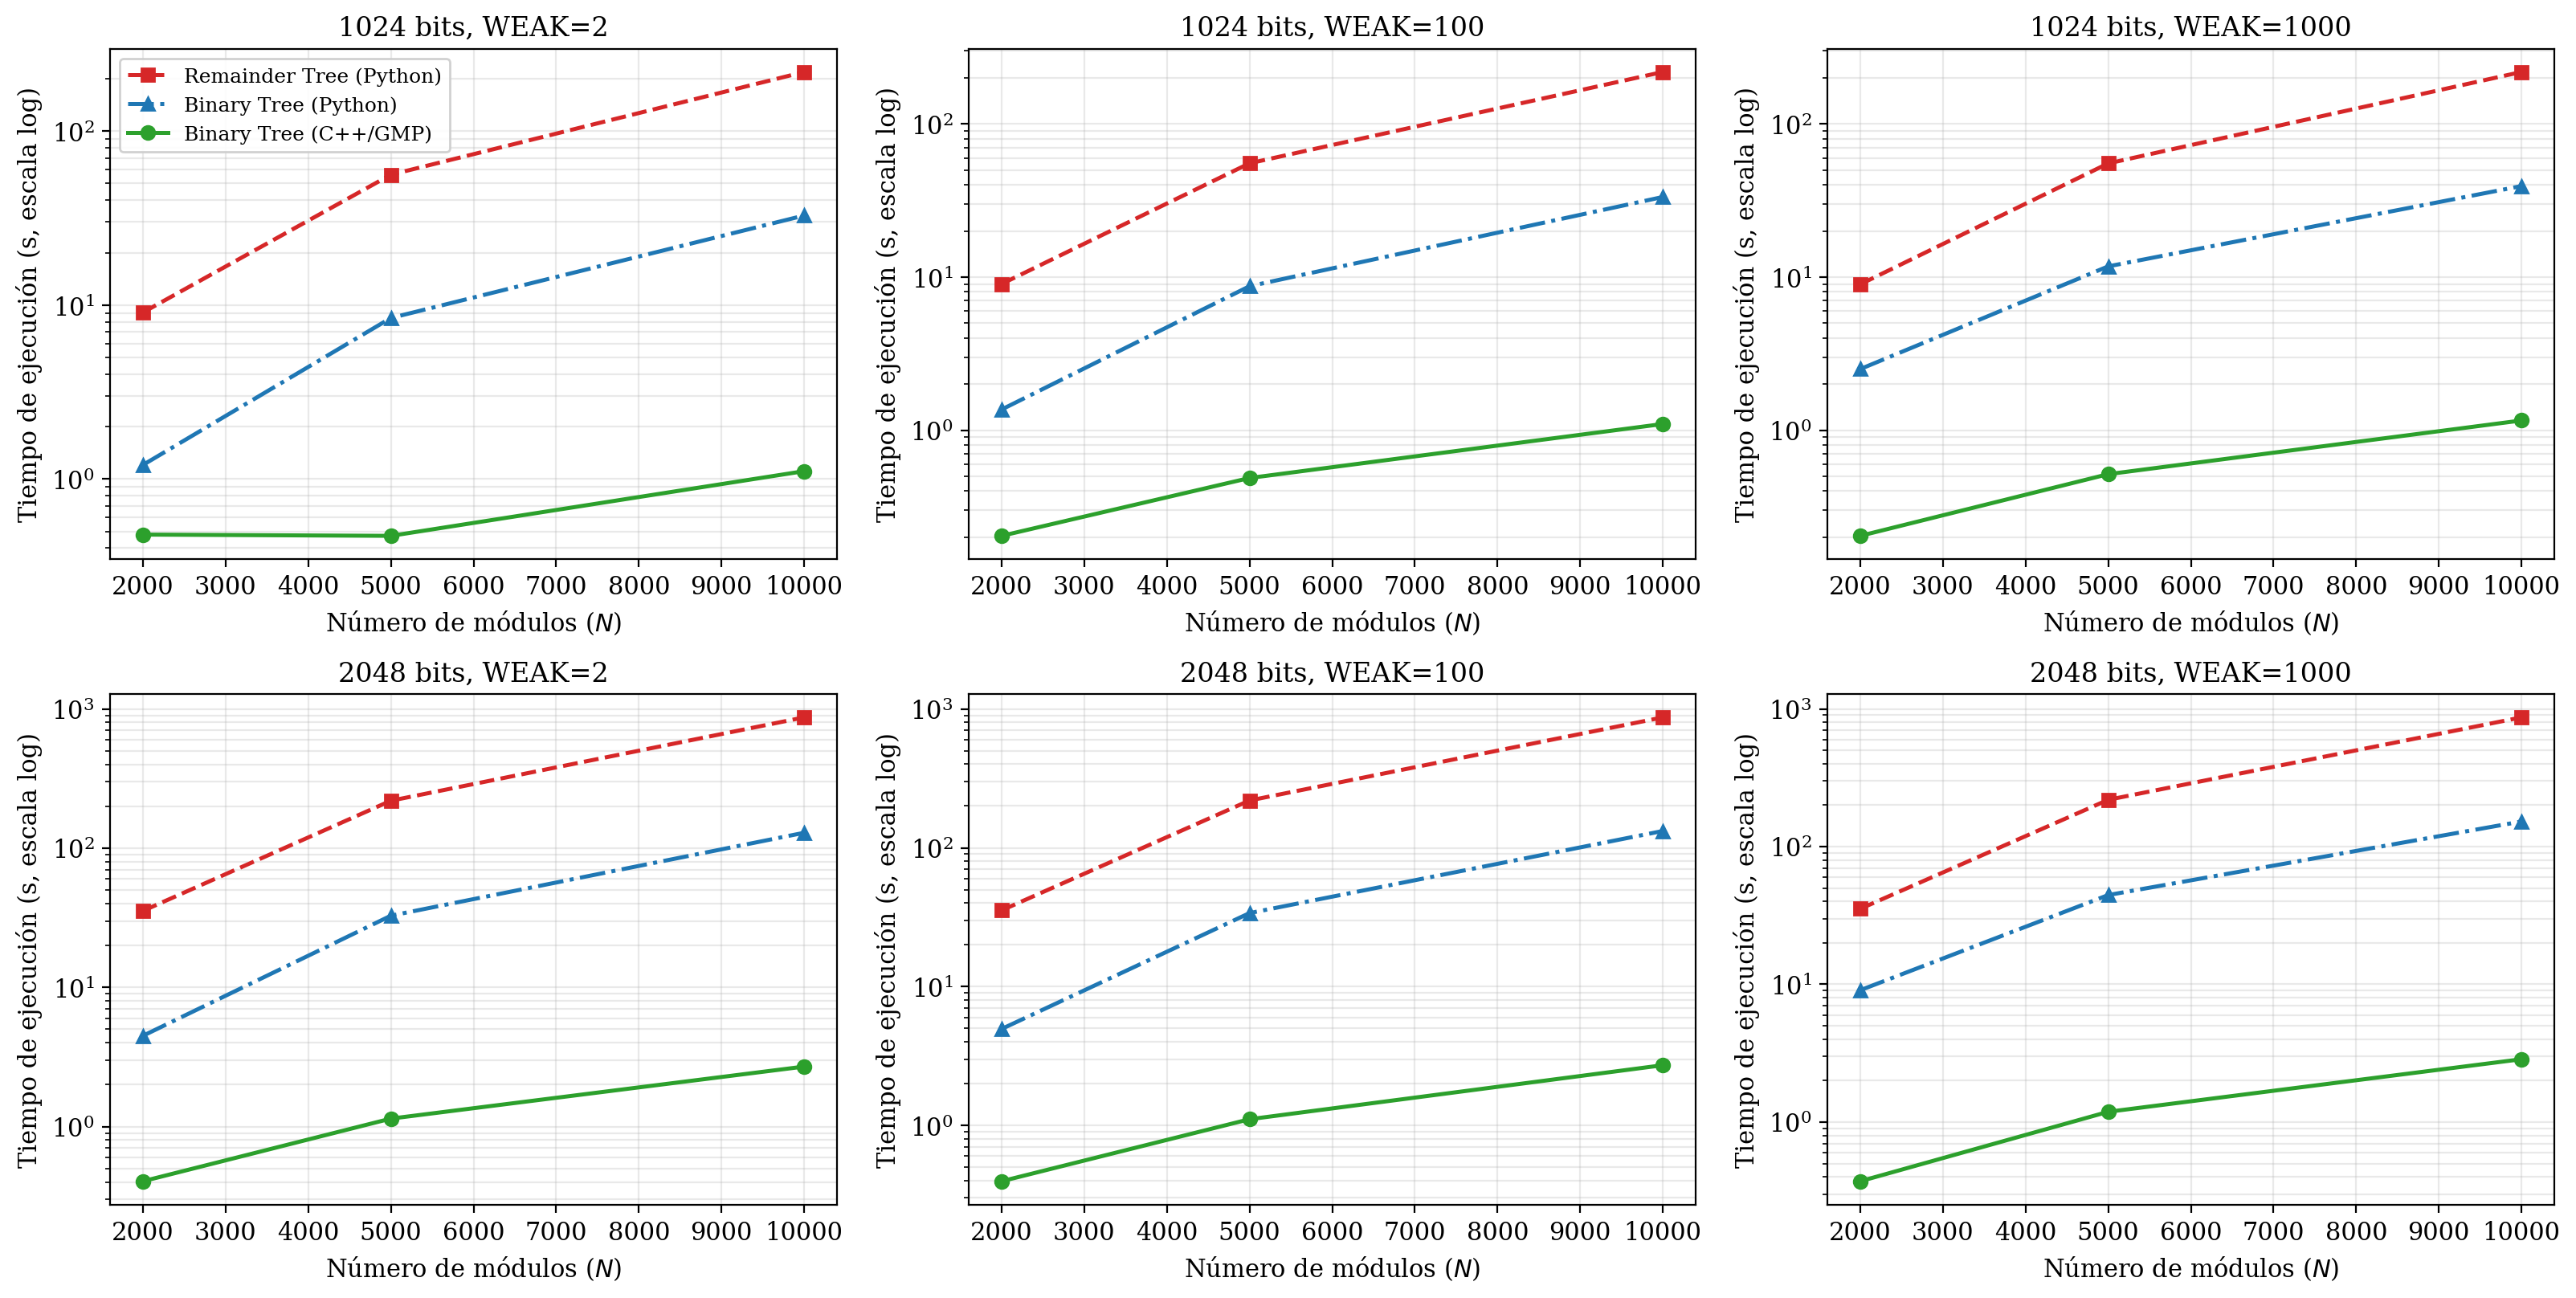
\includegraphics[height=0.66\textheight]{benchmark_tiempo_grid.png}
  \begin{flushleft}\small
  Réplica reducida del experimento de Pelofske (RSA-1024/2048; WEAK = 2, 100, 1000). Escala logarítmica: el orden \alert{Remainder $>$ Binary Python $>$ C++/GMP} se mantiene en todas las configuraciones.
  \end{flushleft}
\end{frame}

\begin{frame}{Comparativa sintética: cifras clave}
  \begin{columns}[T]
    \column{0.52\textwidth}
    \begin{block}{Aceleraciones (media / máx)}
      \small
      \begin{itemize}
        \item Binary Python vs.\ Remainder: \textbf{6,1$\times$} (3,6--7,9)
        \item \textbf{C++/GMP} vs.\ Remainder: \alert{116,5$\times$} (máx \textbf{275,3$\times$})
        \item C++/GMP vs.\ Binary Python: \textbf{18,7$\times$} (máx 41,3$\times$)
      \end{itemize}
    \end{block}
    \column{0.48\textwidth}
    \small
    \begin{tabular}{rrr}
      \toprule
      \multicolumn{3}{c}{\textbf{Caso 2048b, $N{=}10000$, WEAK 1000}}\\
      \midrule
      Remainder Py & Binary Py & C++/GMP \\
      866,8\,s & 152,8\,s & \alert{5,85\,s} \\
      \bottomrule
    \end{tabular}
    \vspace{0.4cm}
    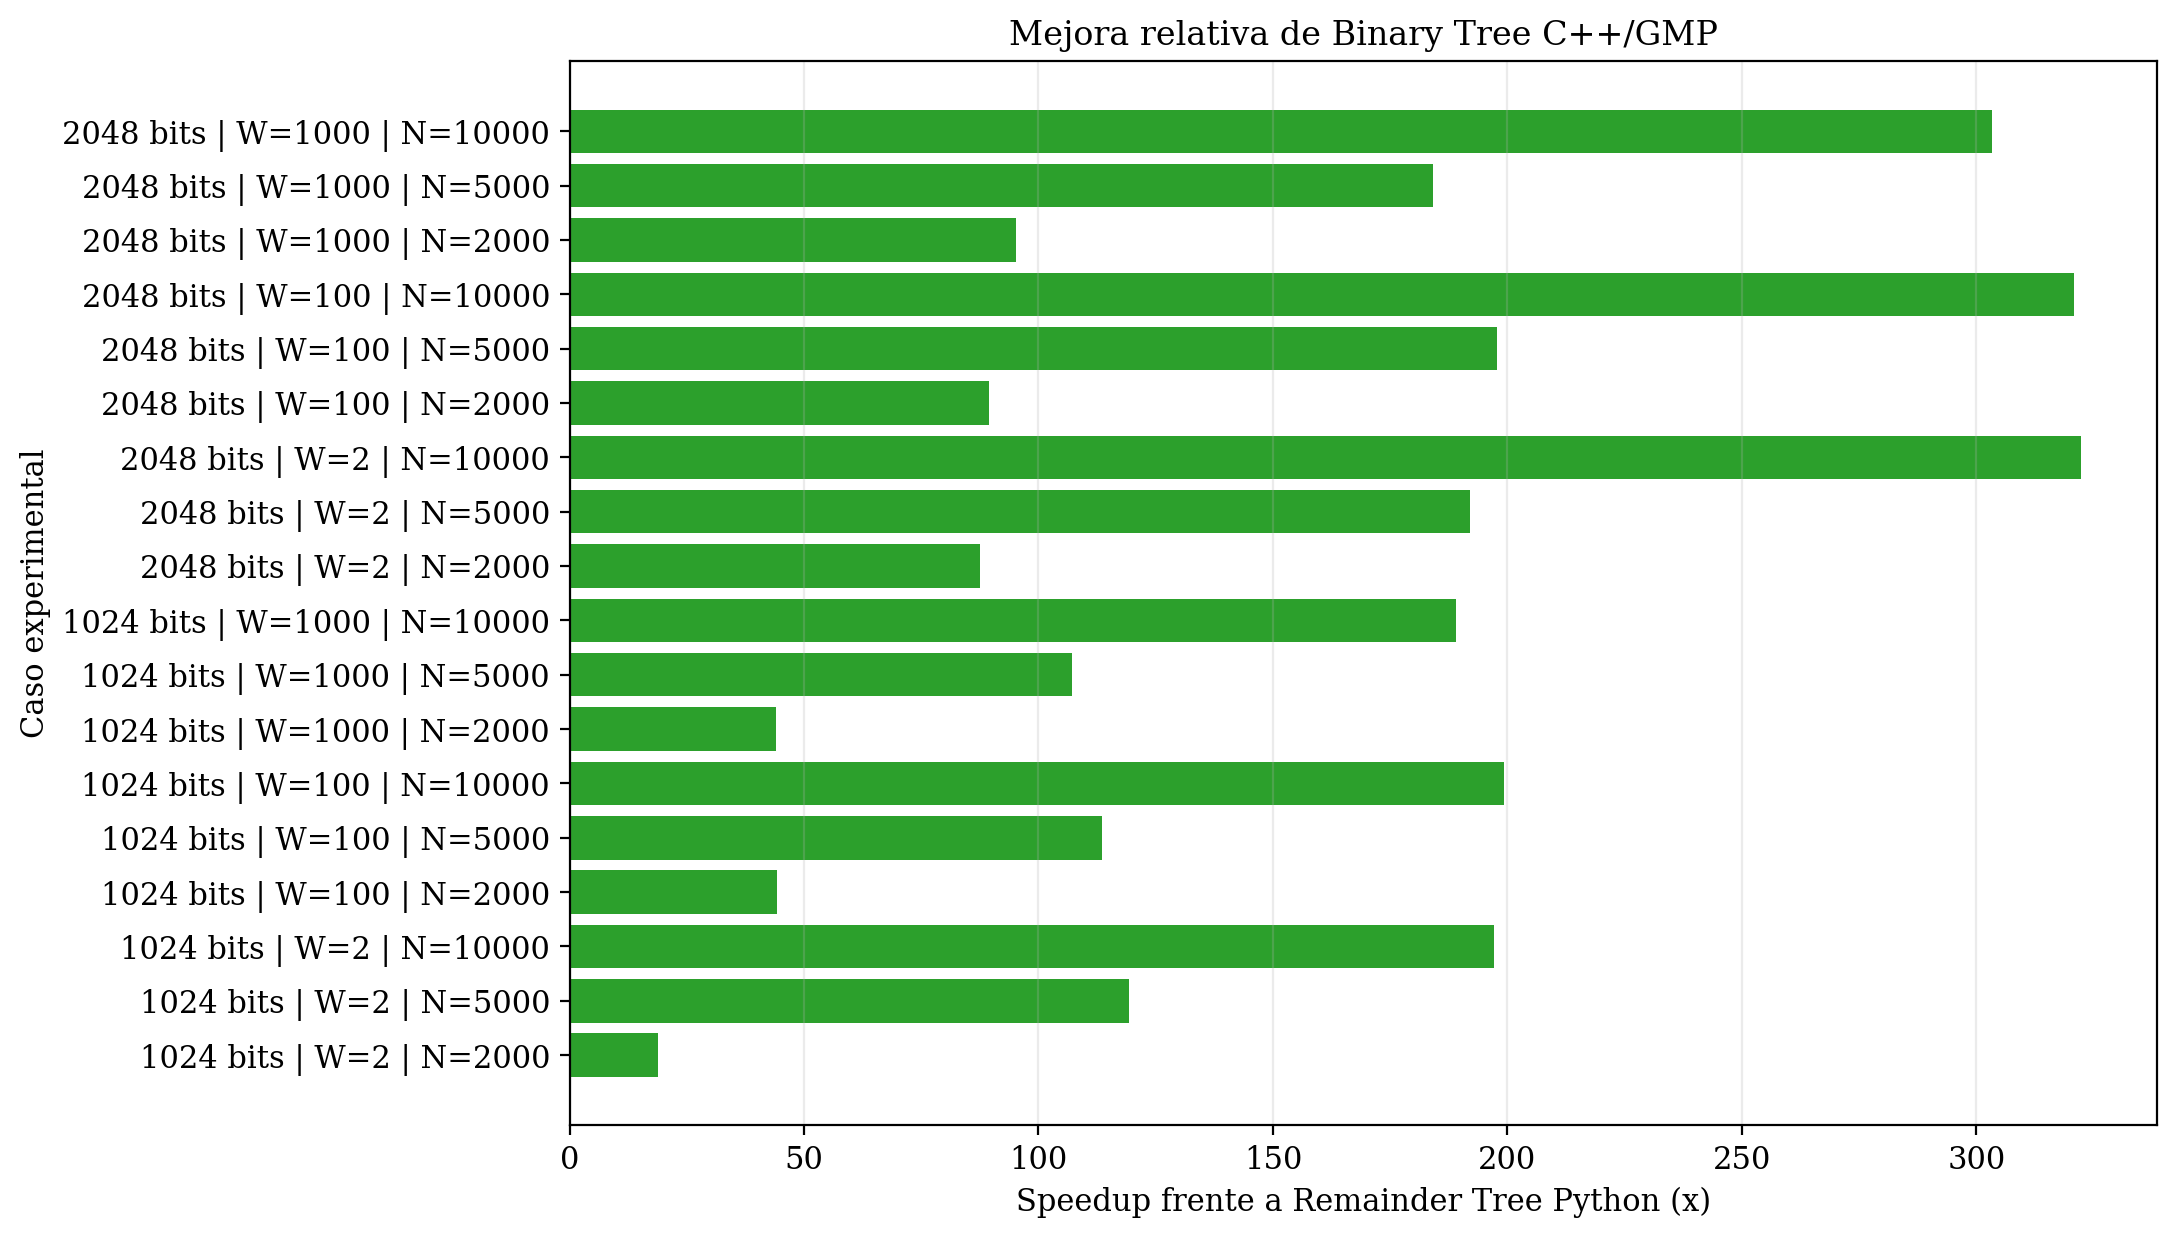
\includegraphics[width=\linewidth]{benchmark_speedup_cpp.png}
  \end{columns}
\end{frame}

\begin{frame}{Comparativa sintética: consumo de memoria}
  \centering
  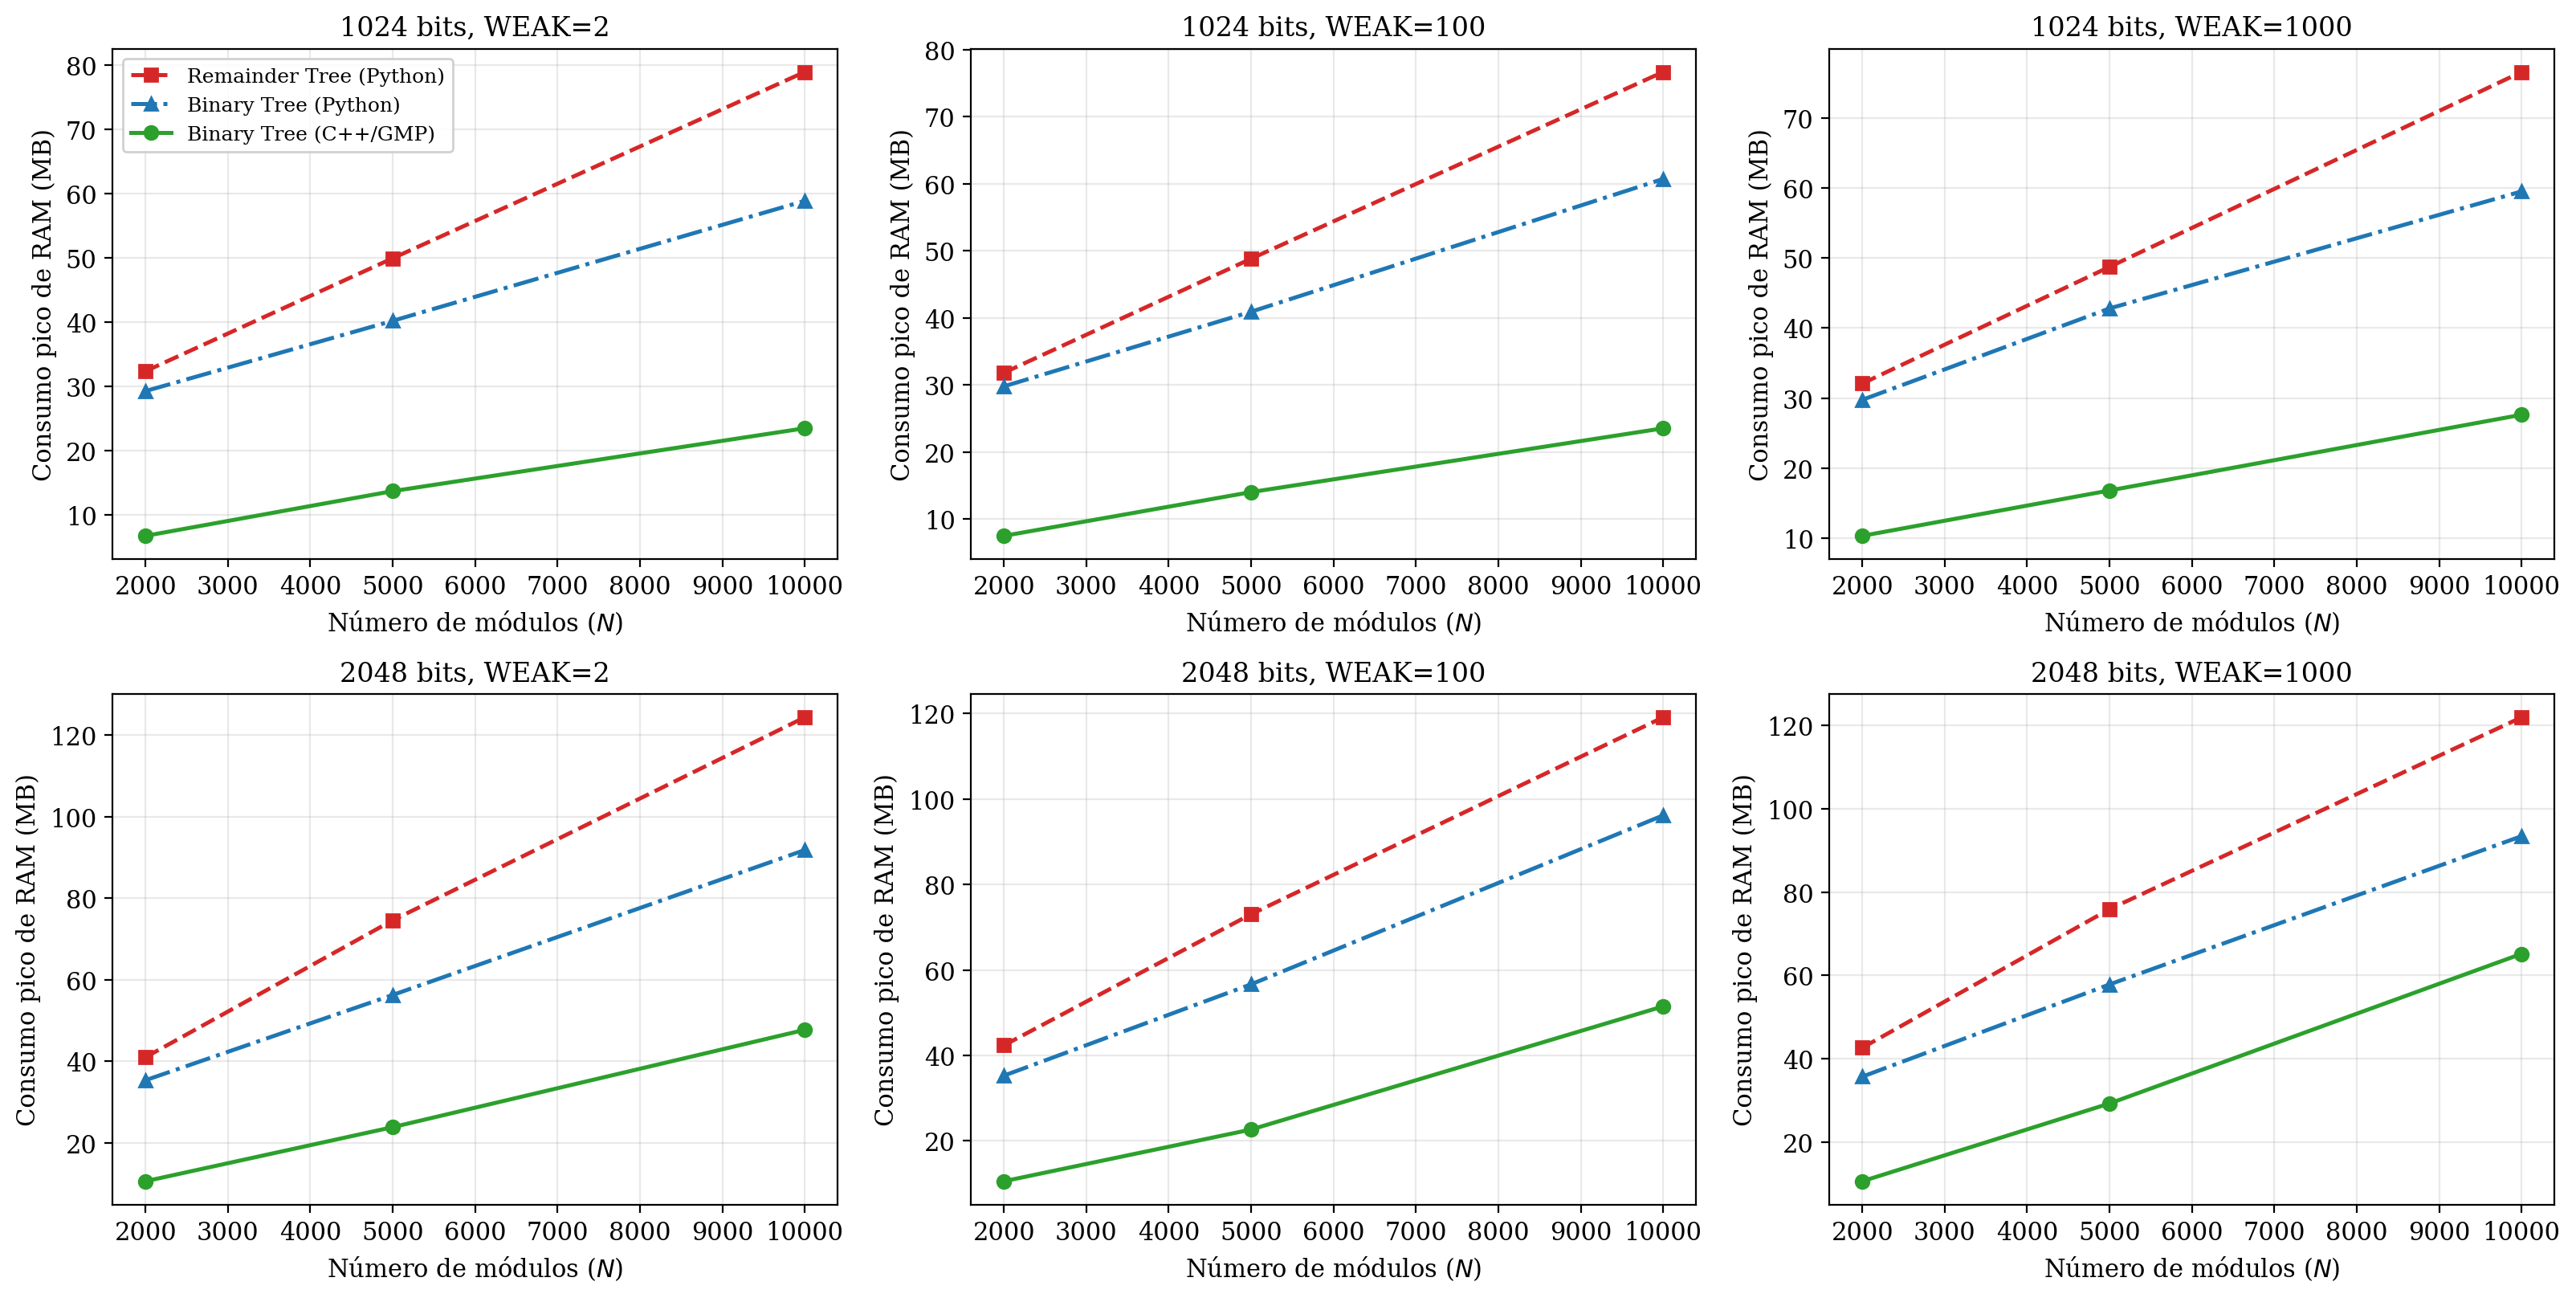
\includegraphics[height=0.6\textheight]{benchmark_memoria_grid.png}
  \begin{flushleft}\small
  Pico de RAM: \textbf{128,7\,MB} (clásico) \;·\; \textbf{94,4\,MB} (Binary Py) \;·\; \alert{57,9\,MB} (C++/GMP).
  Reducción del \textbf{55,0\,\%} frente al clásico y del \textbf{38,7\,\%} frente a Binary Python, gracias a la liberación temprana de nodos.
  \end{flushleft}
\end{frame}

\begin{frame}{Resultados sobre datos reales (CT logs)}
  \begin{columns}[T]
    \column{0.46\textwidth}
    \small
    \begin{tabular}{lr}
      \toprule
      \textbf{Elemento} & \textbf{Valor} \\
      \midrule
      Módulos únicos brutos & 54.278 \\
      Módulos RSA plausibles & \textbf{54.275} \\
      Descartados (validación) & 3 \\
      Logs resumidos & 20 \\
      \textit{GCDs} no triviales & 0 \\
      Claves vulnerables & \textbf{0} \\
      Tiempo total & \alert{$\approx$23,8\,s} \\
      \bottomrule
    \end{tabular}
    \vspace{0.25cm}
    \begin{flushleft}\scriptsize
    Auditoría completa en segundos, frente a los \emph{minutos} de las referencias.
    \end{flushleft}
    \column{0.54\textwidth}
    \centering
    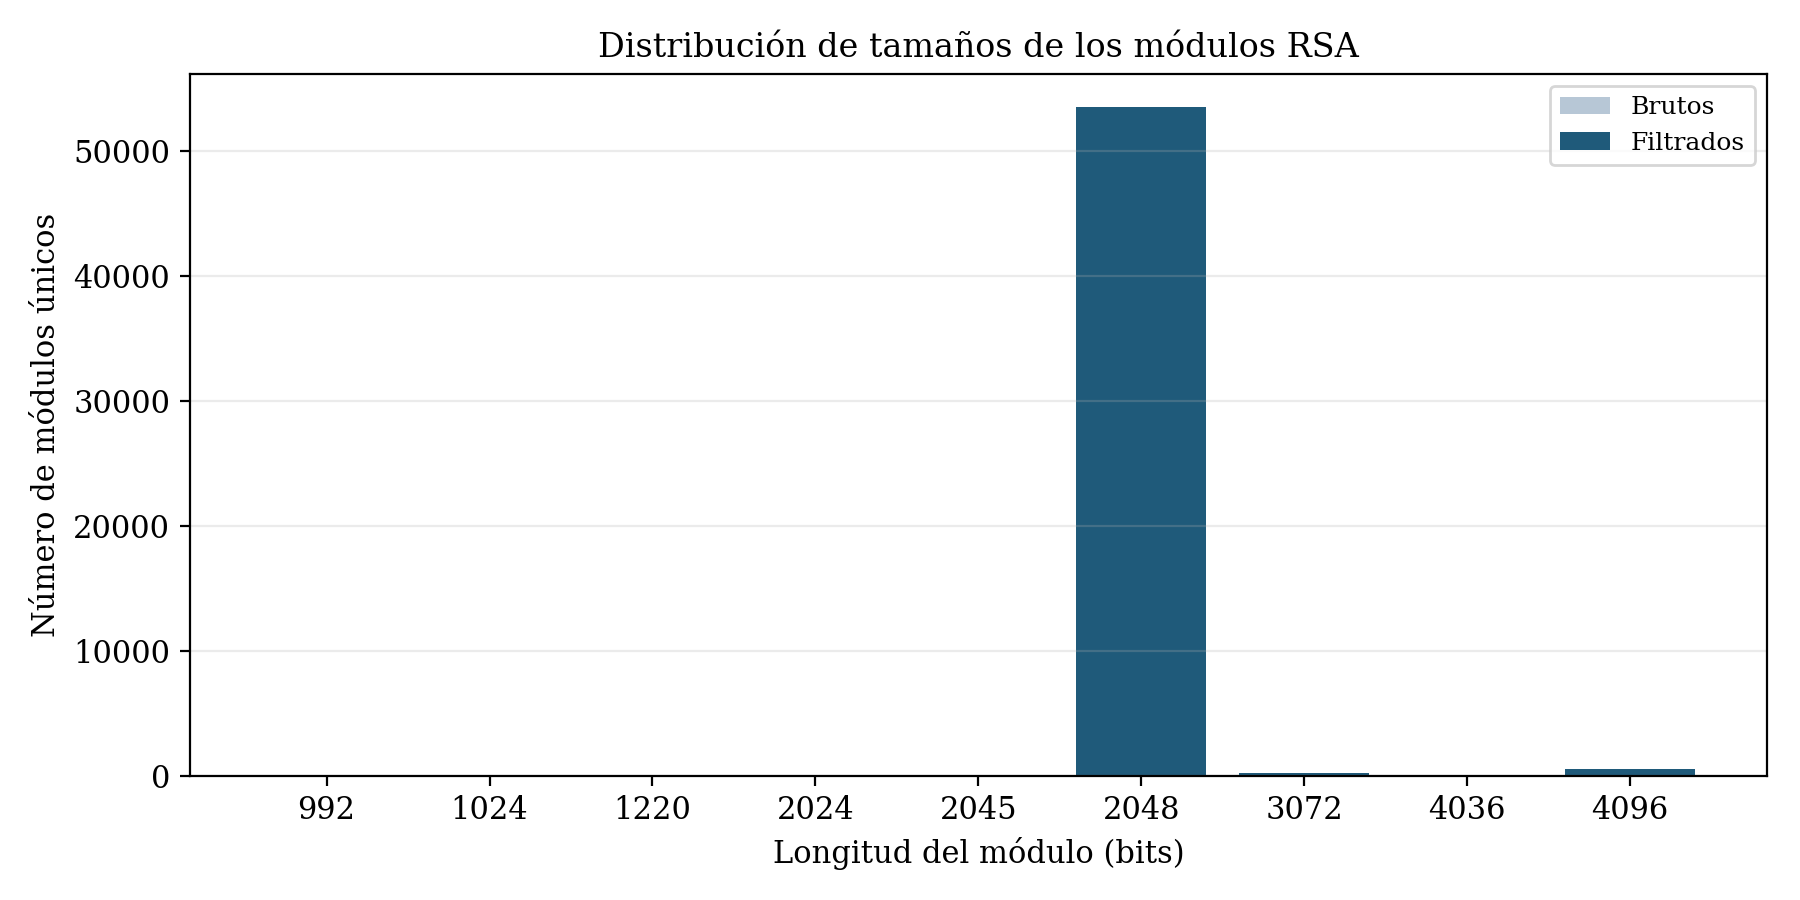
\includegraphics[width=\linewidth]{distribucion_bits_modulos.png}
    \scriptsize Mayoría de claves RSA-2048 (53.539).
  \end{columns}
\end{frame}

%=========================================================================
\section{Conclusiones}

\begin{frame}{Conclusiones}
  \begin{enumerate}
    \item El \textbf{Binary Tree Batch GCD} es una alternativa práctica al enfoque clásico: reduce de forma consistente el tiempo de ejecución.
    \item La \textbf{implementación C++17/GMP} mejora de forma decisiva a las versiones Python (hasta $\sim$275$\times$ en tiempo y $-$55\,\% en memoria).
    \item El comportamiento frente a \texttt{WEAK} encaja con la teoría: ventaja máxima cuando los factores compartidos son \alert{poco frecuentes} (el caso real).
    \item Se entrega un \textbf{flujo completo y reproducible}: extracción, validación, deduplicación y auditoría de módulos reales de CT logs.
  \end{enumerate}
  \vspace{0.15cm}
  \begin{block}{Resultado sobre datos reales}
    \small No se detectaron factores compartidos entre los 54.275 módulos analizados; un resultado \textbf{acotado} al subconjunto extraído, no una garantía global.
  \end{block}
\end{frame}

\begin{frame}{Limitaciones y trabajo futuro}
  \begin{columns}[T]
    \column{0.5\textwidth}
    \textbf{Limitaciones}
    \begin{itemize}\small
      \item Parrilla sintética reducida ($N\le 10000$) por recursos locales.
      \item Una medición por configuración (no estadística).
      \item Conjunto real limitado a certificados de \texttt{issuer/}.
      \item Agregación de $B$ aún secuencial.
    \end{itemize}
    \column{0.5\textwidth}
    \textbf{Trabajo futuro}
    \begin{itemize}\small
      \item Incorporar \textbf{certificados hoja} de las entradas completas.
      \item Paralelizar fases aún secuenciales.
      \item Escalar a conjuntos cercanos a la literatura ($>$100\,M).
    \end{itemize}
  \end{columns}
\end{frame}

%--------------------------- Cierre --------------------------------------
{\setbeamertemplate{footline}{}
\begin{frame}[plain]
  \begin{tikzpicture}[remember picture,overlay]
    \fill[ucazul] (current page.south west) rectangle (current page.north east);
    \fill[ucgranate] ([yshift=1.0cm]current page.south west) rectangle ([yshift=1.15cm]current page.south east);
    \node[anchor=center,text=white,font=\Huge\bfseries] at ([yshift=0.8cm]current page.center) {¡Gracias!};
    \node[anchor=center,text=white,font=\large] at ([yshift=-0.4cm]current page.center) {¿Preguntas?};
    \node[anchor=south,text=ucclaro,font=\small] at ([yshift=1.5cm]current page.south)
      {David Quinzaños Saiz \quad·\quad Binary Tree Batch GCD sobre CT logs \quad·\quad UC--UIMP, 2026};
    \node[anchor=north east,inner sep=14pt] at (current page.north east)
      {
\includegraphics[height=1.0cm]{uc-logo.png}};
  \end{tikzpicture}
\end{frame}
}

\end{document}
